\documentclass[tikz,border=0pt]{standalone}
\usetikzlibrary{positioning,arrows.meta,calc}
\definecolor{cblue}{HTML}{0072B2}
\definecolor{cgreen}{HTML}{009E73}
\definecolor{cgray}{HTML}{555555}
\definecolor{cfill}{HTML}{F4F4F4}
\setlength{\fboxsep}{1.5pt}
\newcommand{\bdg}[2]{\raisebox{-0.2ex}{\colorbox{#1}{\textcolor{white}{\sffamily\bfseries\tiny #2}}}}
\newcommand{\bsimd}{\bdg{cblue}{SIMD}}
\newcommand{\bgpu}{\bdg{cgreen}{GPU}}
\begin{document}
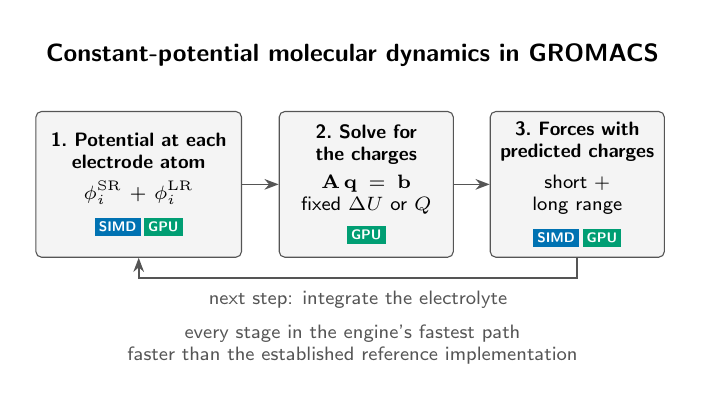
\begin{tikzpicture}[font=\sffamily\scriptsize,
  stage/.style={rounded corners=2pt, draw=cgray, fill=cfill, align=center,
                inner sep=3pt, text width=2.0cm, minimum height=1.85cm},
  arr/.style={-{Stealth[length=1.8mm]}, semithick, draw=cgray}]
\path[use as bounding box] (0,0) rectangle (8.25cm,4.44cm);
\node[font=\sffamily\bfseries\small, anchor=north] at (4.125cm,4.36cm)
  {Constant-potential molecular dynamics in GROMACS};
\node[stage, text width=2.4cm] (pot) at (1.41cm,2.45cm)
  {\textbf{1.\ Potential at each\\electrode atom}\\[3pt]
   $\phi_i^{\mathrm{SR}}+\phi_i^{\mathrm{LR}}$\\[3pt] \bsimd\,\bgpu};
\node[stage] (solve) at (4.30cm,2.45cm)
  {\textbf{2.\ Solve for\\the charges}\\[2pt]
   $\mathbf{A}\,\mathbf{q}=\mathbf{b}$\\[0pt]
   fixed $\Delta U$ or $Q$\\[2pt] \bgpu};
\node[stage] (force) at (6.98cm,2.45cm)
  {\textbf{3.\ Forces with\\predicted charges}\\[3pt]
   short + long range\\[3pt] \bsimd\,\bgpu};
\draw[arr] (pot) -- (solve);
\draw[arr] (solve) -- (force);
\draw[arr] (force.south) -- ++(0,-0.26cm) -| (pot.south)
  node[pos=0.25, below=1pt, text=cgray, font=\sffamily\scriptsize]
  {next step: integrate the electrolyte};
\node[anchor=south, text=cgray, font=\sffamily\scriptsize, align=center] at (4.125cm,0.04cm)
  {every stage in the engine's fastest path\\faster than the established reference implementation};
\end{tikzpicture}
\end{document}
